%\documentclass[12pt,convert={density=150}]{standalone}
\documentclass[12pt]{standalone}

\usepackage{amsmath}
\usepackage{amsfonts}
\usepackage{amssymb}
\usepackage{fontspec}
\usepackage{tikz}

\usetikzlibrary{angles}
\usetikzlibrary{arrows}
\usetikzlibrary{positioning}

\definecolor{juliared}{rgb}{0.796, 0.235, 0.2}
\definecolor{juliagreen}{rgb}{0.22, 0.596, 0.149}
\definecolor{juliablue}{rgb}{0.251, 0.388, 0.847}
\definecolor{juliapurple}{rgb}{0.584, 0.345, 0.698}

\begin{document}
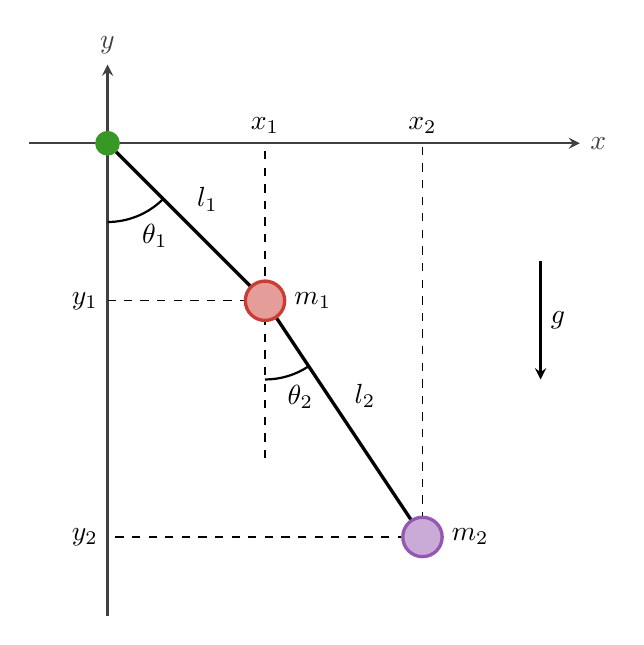
\begin{tikzpicture}

\draw[-stealth, thick, darkgray] (-1,0) -- (6,0) node [right] {$x$};
\draw[-stealth, thick, darkgray] (0,-6) -- (0,1) node [above] {$y$};

\draw[-stealth, thick, black] (5.5,-1.5) --  node [right] {$g$} ++ (0,-1.5);

\draw[very thick, black] (0,0) --  node [above right] {$l_1$} ++ (2,-2);
\draw[very thick, black] (2,-2) -- node [above right] {$l_2$} ++ (2,-3);

\draw[dashed, black] (2,-4) -- (2,0) node [above] {$x_1$};
\draw[dashed, black] (4,-5) -- (4,0) node [above] {$x_2$};

\draw[dashed, black] (2,-2) -- (0,-2) node [left] {$y_1$};
\draw[dashed, black] (4,-5) -- (0,-5) node [left] {$y_2$};

\filldraw[juliagreen] (0,0) circle (0.15);
\filldraw[juliared, fill=juliared!50, very thick] (2,-2) circle (0.25);
\filldraw[juliapurple, fill=juliapurple!50, very thick] (4,-5) circle (0.25);

\draw (2.25,-2) node [right] {$m_1$};
\draw (4.25,-5) node [right] {$m_2$};

\draw[thick] (0,-1) arc (-90:-45:1);% node [midway] {$\theta_1$};
\draw[thick] (2,-3) arc (-90:-56.31:1);% node [midway] {$\theta_2$};

\draw (0.6, -0.9) node [below] {$\theta_1$};
\draw (2.45, -2.95) node [below] {$\theta_2$};

\end{tikzpicture}
\end{document}
